\documentclass{article}

% Official NeurIPS 2025 style (the latest released). [preprint] shows author names;
% the footer is replaced below so the PDF does not claim to be a NeurIPS submission.
\usepackage[preprint]{neurips_2025}
\makeatletter
\renewcommand{\@noticestring}{ESE 5420 course project (University of Pennsylvania, Fall 2026), written in the format of a machine learning paper. Not peer reviewed. Early draft, 16 November 2026.}
\makeatother

\usepackage[utf8]{inputenc}
\usepackage[T1]{fontenc}
\usepackage{hyperref}
\usepackage{url}
\usepackage{booktabs}
\usepackage{amsmath,amsfonts}
\usepackage{microtype}
\usepackage{xcolor}
\usepackage{graphicx}

\newcommand{\todo}[1]{\textcolor{gray}{\textit{[#1]}}}

\title{How Many Training Notes? Sample Efficiency of Logistic Regression,\\ $k$-Nearest Neighbours and Random Forests for Forged-Banknote Detection}

\author{Maanas \And Advit \\ University of Pennsylvania}

\begin{document}
\maketitle

\begin{abstract}
On the UCI Banknote Authentication benchmark, a tuned logistic regression already misclassifies only 0.56\% $\pm$ 0.09\% of notes in 5-fold cross-validation, so comparing methods by final accuracy alone would produce ties. We therefore ask how much labelled data each method needs: we compare logistic regression, $k$-nearest neighbours and random forests along learning curves from 20 to 800 training notes, using 50 random draws per size and tuning every method by cross-validation inside each draw. Early results show a crossover. Logistic regression is the most sample-efficient below about 100 notes (2.5\% vs.\ 4.2\% error for $k$NN at 50 notes), but it levels off near 0.6\%, while $k$NN keeps improving to 0.13\% at 800 notes. \todo{Final numbers, paired differences and the one-time test-set result to be added.}
\end{abstract}

%------------------------------------------------------------------
\section*{Feasibility summary for the early draft}
\begin{itemize}
  \item \textbf{Data acquired and loaded:} 1,372 $\times$ 5 raw table; 1,348 rows after removing 24 exact duplicates; 4 inputs, 1 binary output (Table~\ref{tab:data}).
  \item \textbf{Baseline result:} logistic regression (Module 3) tuned by stratified 5-fold CV (Module 4): \textbf{0.56\% $\pm$ 0.09\%} CV error; nested CV 0.74\% $\pm$ 0.32\% (Table~\ref{tab:baseline}). The baseline uses only material taught before 9 November.
  \item \textbf{Already running:} learning curves for all three methods (Figure~\ref{fig:main}, Table~\ref{tab:learning}). The random forest (Module 7) is the planned extension; no headline result depends on it.
  \item \textbf{Untouched:} the 270-row stratified test set, reserved for one final evaluation.
\end{itemize}

%------------------------------------------------------------------
\section{Introduction \todo{outline}}
\begin{itemize}
  \item Motivation: counterfeit detection is a cheap, low-dimensional classification task. On easy benchmarks, ``which model is most accurate?'' often ends in a tie, while ``which model needs the fewest labelled examples?'' still separates methods.
  \item Question: how many training notes does each method need to reach a given error rate (1\%, 2\%)? Is the answer different for a linear method (logistic regression), a local nonparametric one ($k$NN) and an ensemble (random forest)?
  \item Contributions: (i) a leakage-aware evaluation protocol (duplicate removal, scaling inside folds, an untouched test set, a check for several images per specimen); (ii) paired learning curves with error bars over 50 draws; (iii) an honest statement of where differences are ties.
\end{itemize}

\section{Related work \todo{outline}}
\begin{itemize}
  \item Dataset origin: wavelet features of images of genuine and forged banknote-like specimens \cite{lohweg2012uci,gillich2010banknote}.
  \item Learning curves for comparing classifiers: logistic regression tends to win on small samples and tree induction on large ones, and the curves can cross \cite{perlich2003tree}; discriminative vs.\ generative sample efficiency \cite{ng2002discriminative}; a review of learning-curve shapes \cite{viering2023shape}.
  \item Methods: logistic regression and cross-validation \cite{james2021isl}, nearest neighbours \cite{cover1967nearest}, random forests \cite{breiman2001random}; implementation \cite{pedregosa2011scikit}.
\end{itemize}

%------------------------------------------------------------------
\section{Data}
UCI Banknote Authentication \cite{lohweg2012uci} (CC BY 4.0) contains four features from a wavelet transform of each specimen image: variance, skewness, kurtosis and entropy. There is also a binary class. There are no missing values. We remove 24 exact duplicate rows, all from class 0. UCI does not document which class is forged, and secondary sources disagree. We treat class 1 as forged. Error and AUC do not depend on this choice; forged-class precision and recall would swap.

\begin{table}[h]
  \centering
  \caption{Data size and shape at each stage. ``Forged'' is the share of class 1.}
  \label{tab:data}
  % generated by src/make_tables.py
\begin{tabular}{lrrr}
\toprule
Stage & Rows & Inputs & Forged \\
\midrule
Raw UCI file & 1372 & 4 & 44.5\% \\
After removing exact duplicates & 1348 & 4 & 45.3\% \\
Development set (80\%) & 1078 & 4 & 45.3\% \\
Test set (20\%, held out) & 270 & 4 & 45.2\% \\
\bottomrule
\end{tabular}
% 24 duplicate rows dropped

  \vspace{4pt}

  \small First rows of the cleaned table (two per class):\\[2pt]
  % generated by src/make_tables.py
\begin{tabular}{rrrrc}
\toprule
Variance & Skewness & Kurtosis & Entropy & Class \\
\midrule
3.622 & 8.666 & -2.807 & -0.447 & 0 \\
4.546 & 8.167 & -2.459 & -1.462 & 0 \\
-1.397 & 3.319 & -1.393 & -1.995 & 1 \\
0.390 & -0.143 & -0.032 & 0.351 & 1 \\
\bottomrule
\end{tabular}

\end{table}

%------------------------------------------------------------------
\section{Method}
\paragraph{Split.} A stratified 80/20 split (seed 5420) gives 1,078 development rows and 270 test rows. The split is stored in \texttt{data/split.csv}, and the analysis code only ever loads the development rows.

\paragraph{Models and tuning.} Each model is a scikit-learn pipeline, so standardisation is fitted on each training fold only. Logistic regression tunes $C \in \{10^{-3}, 10^{-2.5}, \dots, 10^{3}\}$, $k$NN tunes $k \in \{1,3,5,7,9,11,15,21,31\}$, and the random forest (200 trees) tunes \texttt{max\_features} $\in\{1,2,4\}$ and \texttt{min\_samples\_leaf} $\in\{1,3\}$. Hyperparameters are always chosen by stratified 5-fold CV on training data only.

\paragraph{Learning curves.} For $n \in \{20, 50, 100, 200, 400, 800\}$ we draw 50 stratified training sets of size $n$ from the development data. In each draw we tune every method by 5-fold CV inside the training set and score it on all remaining development rows. All methods share the same draws, so the comparison is paired.

\paragraph{Specimen leakage check.} The file has no specimen identifiers. However, class-1 rows show strong serial correlation in file order (lag-1 autocorrelation of skewness 0.62, against about 0 for class 0), which suggests several images per specimen. As a check, we re-ran CV with each run of 8 consecutive rows kept in one fold (\texttt{StratifiedGroupKFold}). The errors were unchanged: logistic regression 0.65\% in both cases, $k$NN 0.09\% in both cases.

%------------------------------------------------------------------
\section{Results so far}
\begin{table}[h]
  \centering
  \caption{Baseline on the development data (test set untouched). SE is the standard error of the five fold errors, SD$/\sqrt{5}$. The 95\% interval is a Wilson interval on the pooled out-of-fold errors.}
  \label{tab:baseline}
  \small
  % generated by src/make_tables.py
\begin{tabular}{lrrl}
\toprule
Model / estimate & Error & SE & Notes \\
\midrule
Majority class & 45.3\% & -- & -- \\
Logistic regression, $C=100$ (5-fold CV) & 0.56\% & 0.09\% & 6/1078; 95\% CI 0.26\%--1.21\% \\
Logistic regression, nested 5$\times$5 CV & 0.74\% & 0.32\% & AUC 0.9999 \\
Logistic regression, 10 repeats of 5-fold & 0.54\% & -- & range 0.37\%--0.65\% \\
\bottomrule
\end{tabular}

\end{table}

\begin{figure}[h]
  \centering
  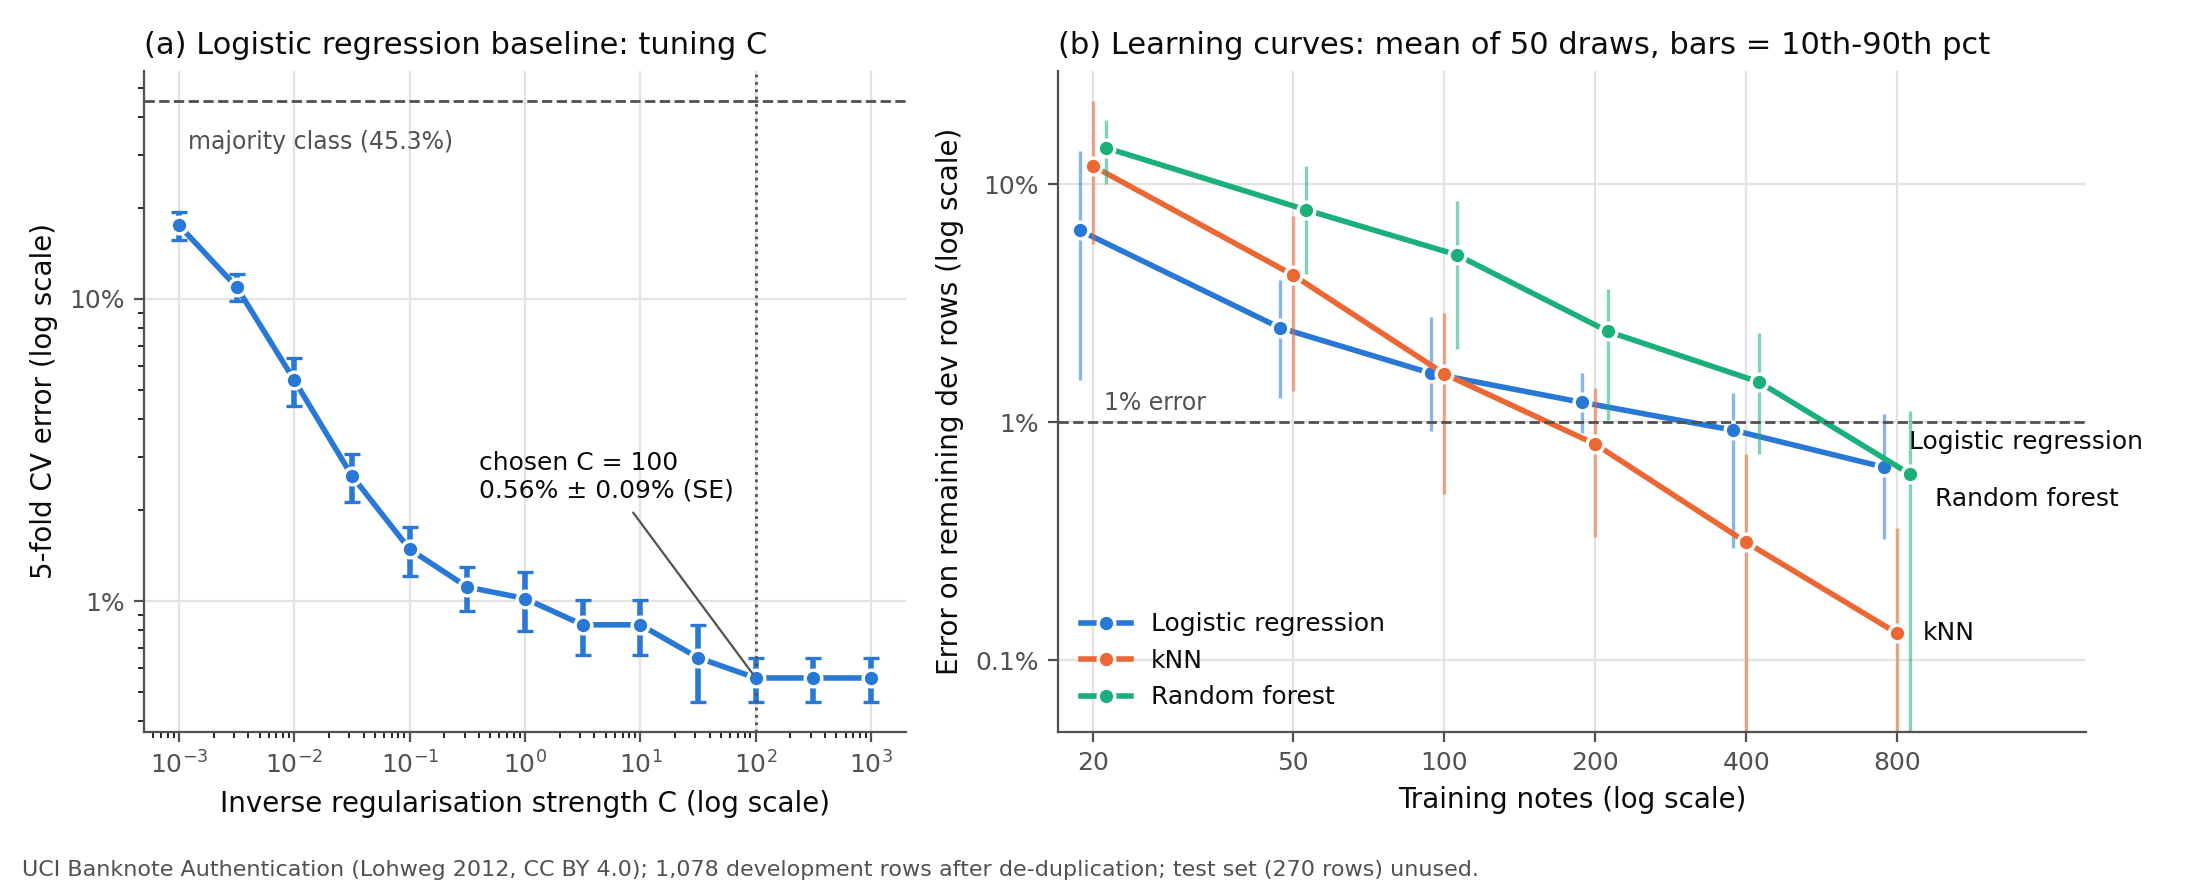
\includegraphics[width=\linewidth]{../figures/baseline.png}
  \caption{(a) Logistic-regression CV error across the $C$ grid, with $\pm1$ SE bars. (b) Learning curves: mean error on held-out development rows over 50 draws; bars show the 10th--90th percentiles across draws.}
  \label{fig:main}
\end{figure}

\begin{table}[h]
  \centering
  \caption{Learning curves: mean error (\%) $\pm$ SE over 50 draws on the remaining development rows. Bold marks the lowest mean; gaps within about 2 SE (e.g.\ $n=100$) are ties. $^\dagger$Module 7 extension.}
  \label{tab:learning}
  \small
  % generated by src/make_tables.py
\begin{tabular}{rccc}
\toprule
$n$ & Logistic regression & $k$NN & Random forest$^\dagger$ \\
\midrule
20 & \textbf{6.39 $\pm$ 0.85} & 11.89 $\pm$ 1.04 & 14.22 $\pm$ 0.71 \\
50 & \textbf{2.50 $\pm$ 0.20} & 4.15 $\pm$ 0.35 & 7.81 $\pm$ 0.45 \\
100 & 1.61 $\pm$ 0.11 & \textbf{1.60 $\pm$ 0.15} & 5.05 $\pm$ 0.34 \\
200 & 1.21 $\pm$ 0.06 & \textbf{0.81 $\pm$ 0.07} & 2.41 $\pm$ 0.15 \\
400 & 0.93 $\pm$ 0.05 & \textbf{0.31 $\pm$ 0.04} & 1.47 $\pm$ 0.09 \\
800 & 0.65 $\pm$ 0.06 & \textbf{0.13 $\pm$ 0.03} & 0.60 $\pm$ 0.06 \\
\bottomrule
\end{tabular}

\end{table}

\paragraph{Reading so far.} Logistic regression needs about 400 notes to reach 1\% mean error, $k$NN about 200, and the random forest between 400 and 800. Cross-validation picks $k=1$ at every size, which is consistent with near-duplicate images of the same specimen. Even so, the grouped check above shows no change in error.

%------------------------------------------------------------------
\section{Remaining sections \todo{outline}}
\paragraph{Experiments to finish (by 30 November).}
\begin{itemize}
  \item Add sizes $n\in\{10, 30, 150, 300, 600\}$; report paired differences ($k$NN $-$ LR, RF $-$ LR) with SE and the share of draws each method wins.
  \item Estimate $n$ needed to reach 1\% and 2\% error for each method, with a bootstrap interval over draws.
  \item Extension (Module 7): tune the forest more fully (trees, OOB error), and add boosting if time allows.
  \item One final evaluation on the 270-row test set, with confusion matrices and ROC curves. Report it as a tie where the SE ($\approx$0.4--0.6\%) says so.
\end{itemize}
\paragraph{Discussion and limitations.} Why a linear boundary saturates and $k$=1 keeps improving on these features. Conclusions are limited to this benchmark, not to real-world currency authentication. We cover the label-coding ambiguity, specimen leakage that cannot be fully tested, overlap between the evaluation sets of different draws, and the small test set.
\paragraph{Conclusion.} One paragraph answering the sample-size question.

\section*{Contributions and AI use \todo{draft}}
Maanas built the data pipeline, the baseline and the learning-curve experiments. Advit will lead the random-forest extension and the evaluation plots. Both write the paper. We used an LLM assistant (Claude) for code generation, debugging and copy-editing. All experimental results were produced and checked by the authors. Code: \url{https://github.com/maanasgoel/ese5420-banknote}.

\bibliographystyle{plain}
\begin{thebibliography}{10}
\bibitem{lohweg2012uci} V.~Lohweg. Banknote Authentication. UCI Machine Learning Repository, 2012. \url{https://archive.ics.uci.edu/dataset/267/banknote+authentication}. CC BY 4.0.
\bibitem{gillich2010banknote} E.~Gillich and V.~Lohweg. Banknotenauthentifizierung. In \emph{1. Jahreskolloquium ``Bildverarbeitung in der Automation''}, Lemgo, Germany, 2010.
\bibitem{perlich2003tree} C.~Perlich, F.~Provost, and J.~S. Simonoff. Tree induction vs.\ logistic regression: A learning-curve analysis. \emph{Journal of Machine Learning Research}, 4:211--255, 2003.
\bibitem{ng2002discriminative} A.~Y. Ng and M.~I. Jordan. On discriminative vs.\ generative classifiers: A comparison of logistic regression and naive Bayes. In \emph{Advances in Neural Information Processing Systems 14}, 2002.
\bibitem{viering2023shape} T.~Viering and M.~Loog. The shape of learning curves: A review. \emph{IEEE Transactions on Pattern Analysis and Machine Intelligence}, 45(6):7799--7819, 2023.
\bibitem{james2021isl} G.~James, D.~Witten, T.~Hastie, and R.~Tibshirani. \emph{An Introduction to Statistical Learning}. Springer, 2nd edition, 2021.
\bibitem{cover1967nearest} T.~Cover and P.~Hart. Nearest neighbor pattern classification. \emph{IEEE Transactions on Information Theory}, 13(1):21--27, 1967.
\bibitem{breiman2001random} L.~Breiman. Random forests. \emph{Machine Learning}, 45(1):5--32, 2001.
\bibitem{pedregosa2011scikit} F.~Pedregosa et al. Scikit-learn: Machine learning in Python. \emph{Journal of Machine Learning Research}, 12:2825--2830, 2011.
\end{thebibliography}

\end{document}
